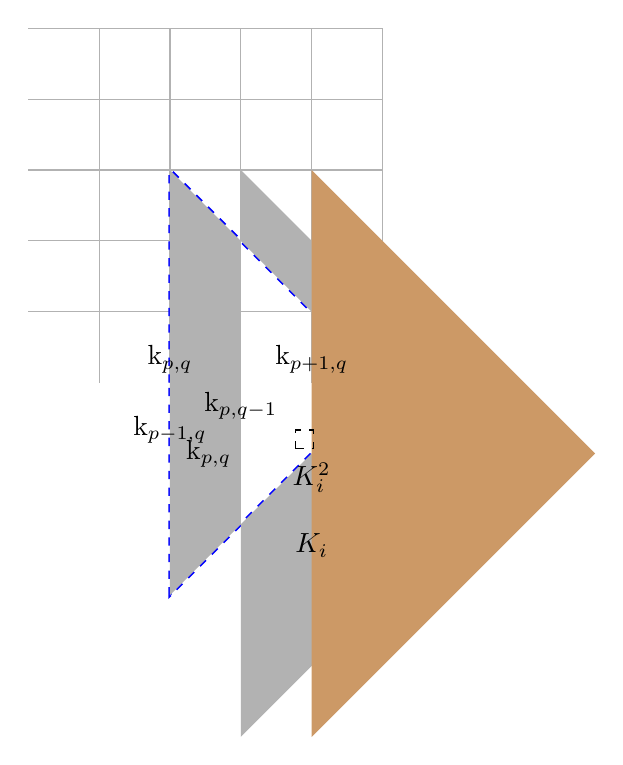
\begin{tikzpicture}[scale=.9]

\foreach \i in {0,...,4} {
    \draw[black!30] (\i,-1)--+(0,5);
    \draw[black!30] (-1,\i)--+(5,0);
}
\draw[dashed,very thick,blue] (1,-1)--+(0,3)--+(3,0)--+(0,-3)--cycle;
\fill[gray!60,even odd rule]
    (2,-2)--+(0,4)--+(4,0)--+(0,-4)--cycle
    (1,-1)--+(0,3)--+(3,0)--+(0,-3)--cycle;
\fill[brown!80] (3,-2)--+(0,4)--+(4,0)--+(0,-4)--cycle;
\path
    (2,-2) coordinate(label_1)
    (1,-1) coordinate[label=$\mathrm{k}_{p,q}$](label_2)
    (2,-1) coordinate[label=below:$\mathrm{k}_{p,q-1}$](label_3)
    (3,-1) coordinate[label=above:$\mathrm{k}_{p+1,q}$](label_4)
    (2,-2) coordinate[label=left:$\mathrm{k}_{p,q}$](label_5)
    (1,-2) coordinate[label=above:$\mathrm{k}_{p-1,q}$](label_6)
    (3,-2) coordinate[label=below:$K_i^2$](label_7)
    (3,-3) coordinate[label=below:$K_i$](label_8)
    (label_8|-label_7) coordinate(north_right_corner)
    (north_right_corner)++(-.1,.2) coordinate(dotted_right_upper_corner);
\node[draw,dashed] at (dotted_right_upper_corner){};
\end{tikzpicture}